\chapter{Appendix For Is a More Accessible Local Government a More Representative One? The Effects of Online Public Meetings}
\label{app:Chapter1}
\SingleSpacing*
\setSingleSpace{1.15}

    \section{Additional Sample Details:}
    Within the section below, I include details of my primary sample of local governments, including their names, socio-economic makeup, and meeting access over the course of my study.
    
    \subsection{Included Local Governments:}
    The subsection below details the local governments included within my sample. Meeting minutes were gathered from each government's official website or data repository.\\\\
    County:
    \begin{itemize}
      \item St. Louis County Government
    \end{itemize}
    Cities:
    \begin{multicols}{2}
      \begin{itemize}
        \item St. Ann
        \item Richmond Heights
        \item Kirkwood
        \item Ellisville
        \item Creve Coeur
        \item Brentwood
        \item Chesterfield
        \item Maplewood
        \item Ballwin
        \item Bridgeton
        \item Hazelwood
        \item Des Peres
        \item Manchester
      \end{itemize}
    \end{multicols}
    
  \noindent School Districts:
    \begin{multicols}{2}
    \begin{itemize}
      \item Parkway SD
      \item Kirkwood SD
      \item Brentwood SD
      \item Ferguson-Florissant SD
      \item Pattonville SD
      \item Hazelwood SD
      \item Ritenour SD
      \item Riverview Gardens SD
      \item Ladue SD
      \item Affton SD
      \item University City SD
      \item Clayton SD
      \item Rockwood SD
      \item Webster Groves SD
      \item Maplewood-Richmond Heights SD
    \end{itemize}
    \end{multicols}
    


    \subsection{Demographic Characteristics:}

    All of the following demographic estimates come from the 2020 American Community Survey.

    \begin{table}[H] \centering 
      \caption{Average Demographic Characteristics of Sample Governments} 
      \label{} 
      \scalebox{0.85}{\begin{tabular}{@{\extracolsep{5pt}} llll} 
    \\[-1.8ex]\hline 
    \hline \\[-1.8ex] 
    Variable & County & City & School \\ 
    \hline
    \\[-1.8ex] 
    Population & 1001982.00 &   21051.55 &   52118.20 \\ 
    Gender (F) & 47.77 & 47.51 & 47.68 \\ 
    White & 65.25 & 65.70 & 65.30 \\ 
    Black & 24.18 & 22.59 & 22.80 \\ 
    Asian & 4.55 & 4.87 & 5.12 \\ 
    Other & 1.36 & 1.79 & 1.67 \\ 
    Age (45+)  & 44.41 & 43.38 & 42.07 \\ 
    Education (College+) & 45.29 & 48.10 & 51.42 \\ 
    Median Income & 72562.00 & 81979.77 & 82670.27 \\ 
    Per Capita Income & 45307.00 & 46662.45 & 49951.33 \\ 
    Gini Index & 0.50 & 0.44 & 0.46 \\ 
    Median Structure Year & 1968 & 1966 & 1961 \\ 
    \hline \\[-1.8ex] 
    \end{tabular} }
    \end{table}

    \subsection{Access By Level of Government}
    \begin{figure}[H]
      \centering
       \text{Access to City Meetings From 2018-2021}\par\medskip
      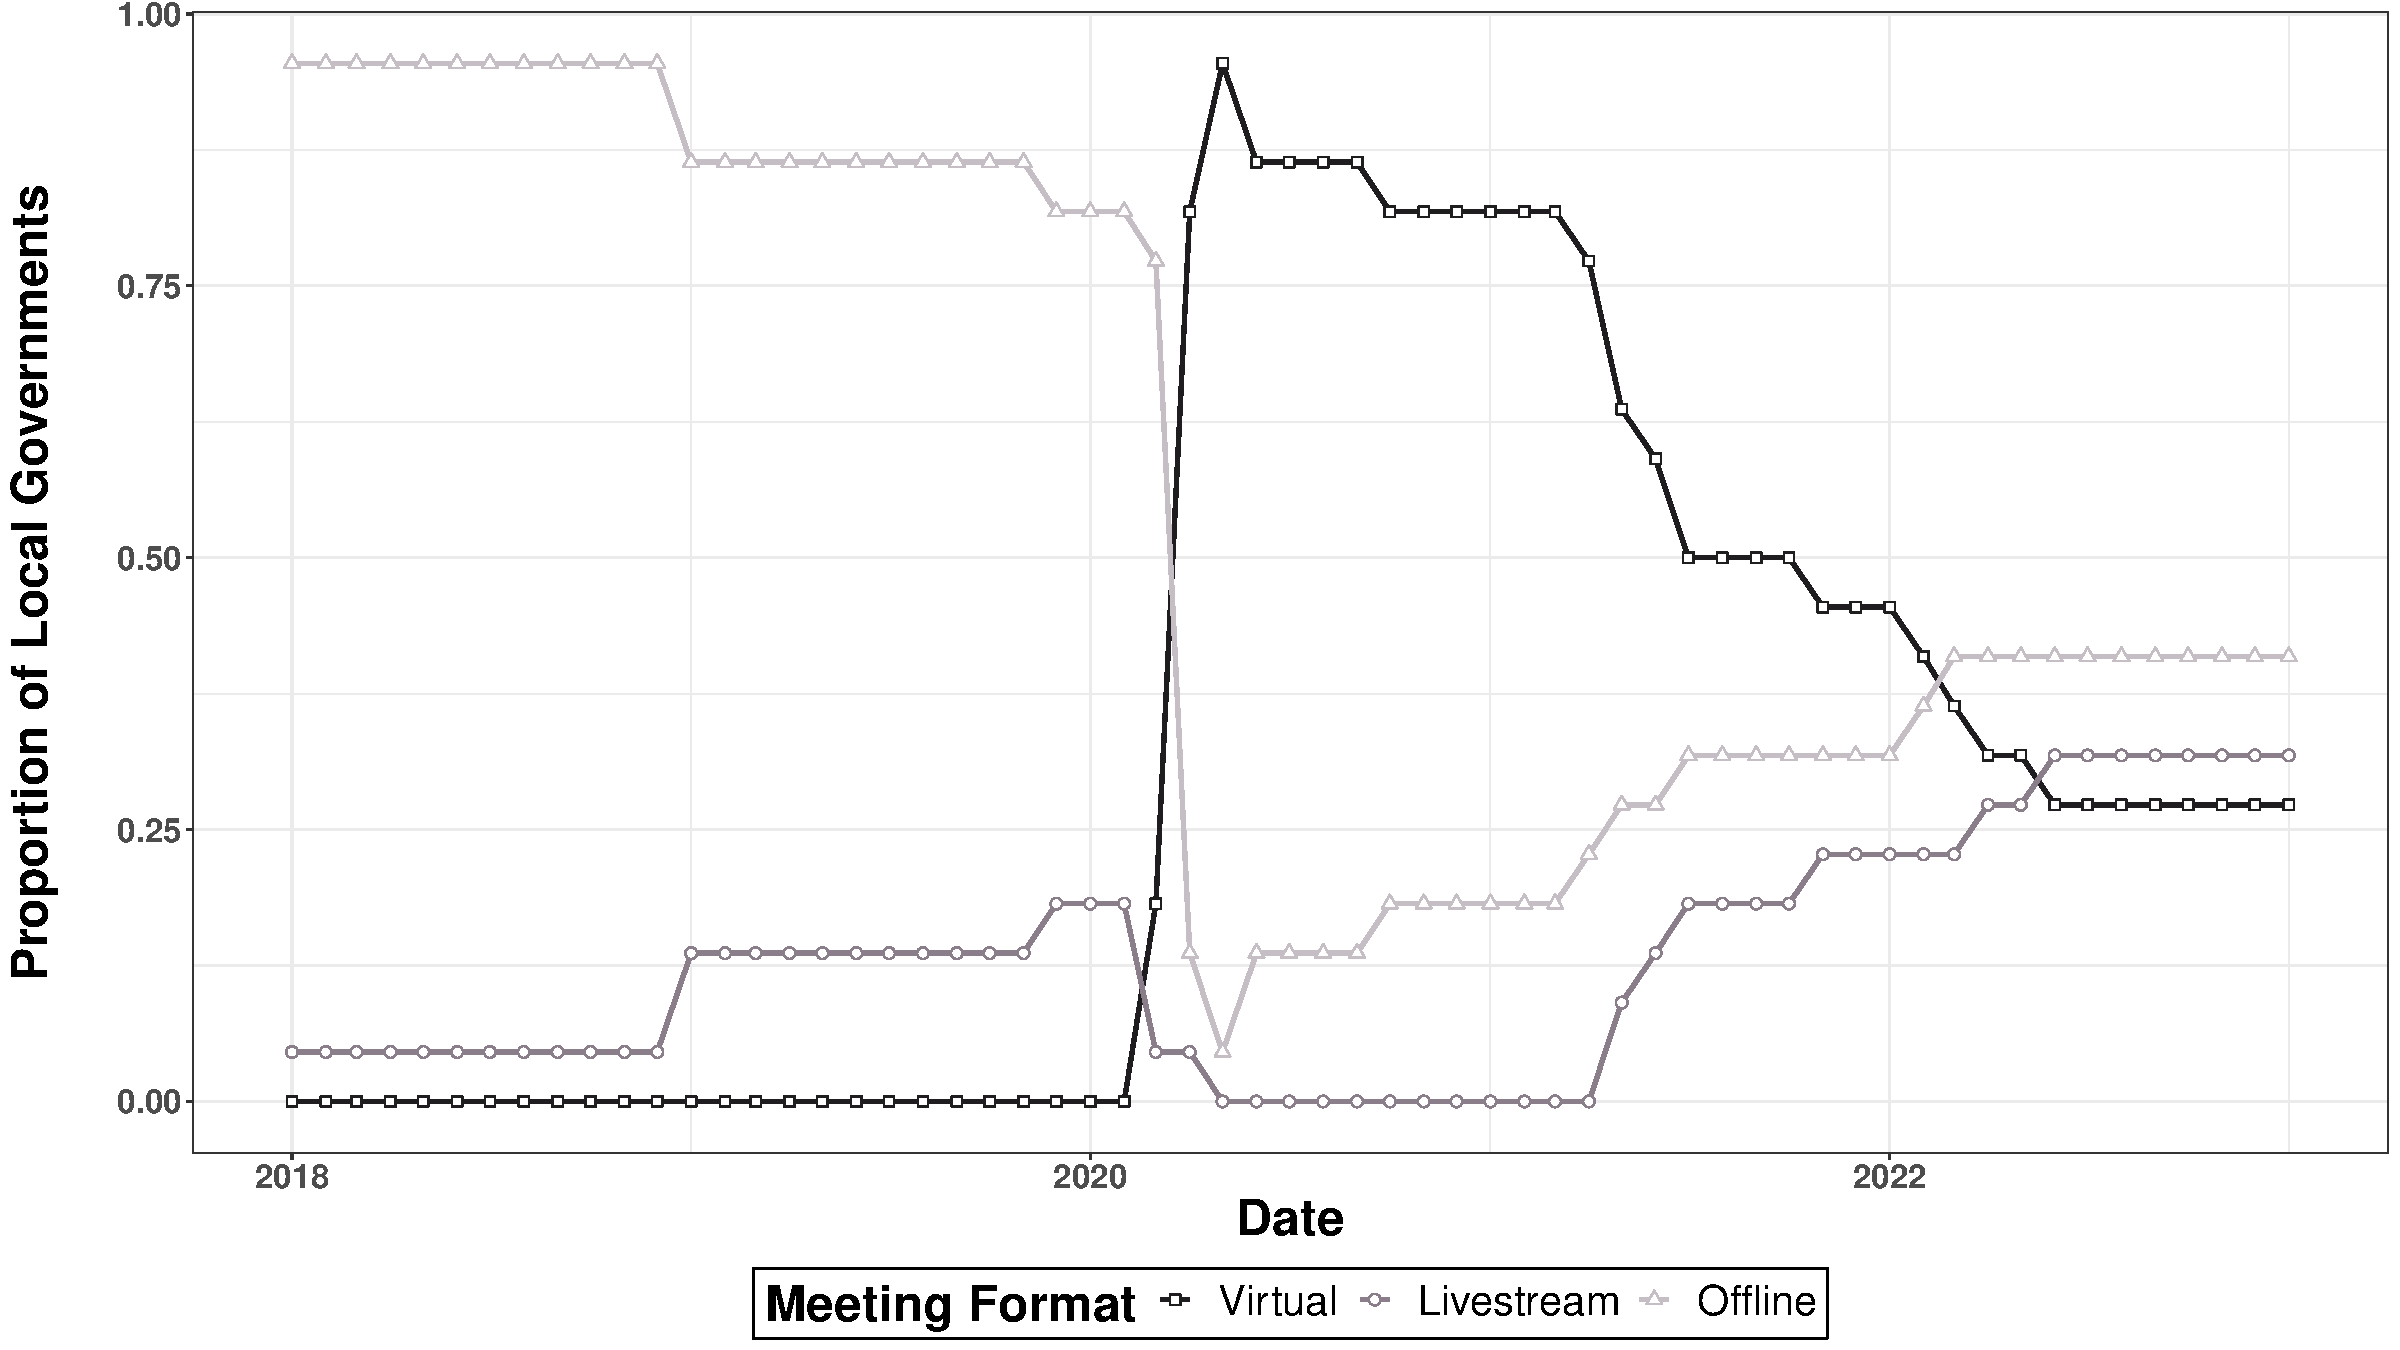
\includegraphics[scale=0.3]{Figures/CityAccess.pdf}
      \caption[Access to City Meetings From 2018-2021]{\footnotesize{Access to City Meetings From 2018-2021}}
      \label{}
  \end{figure}

  \begin{figure}[H]
    \centering
     \text{Access to School Board Meetings From 2018-2022}\par\medskip
    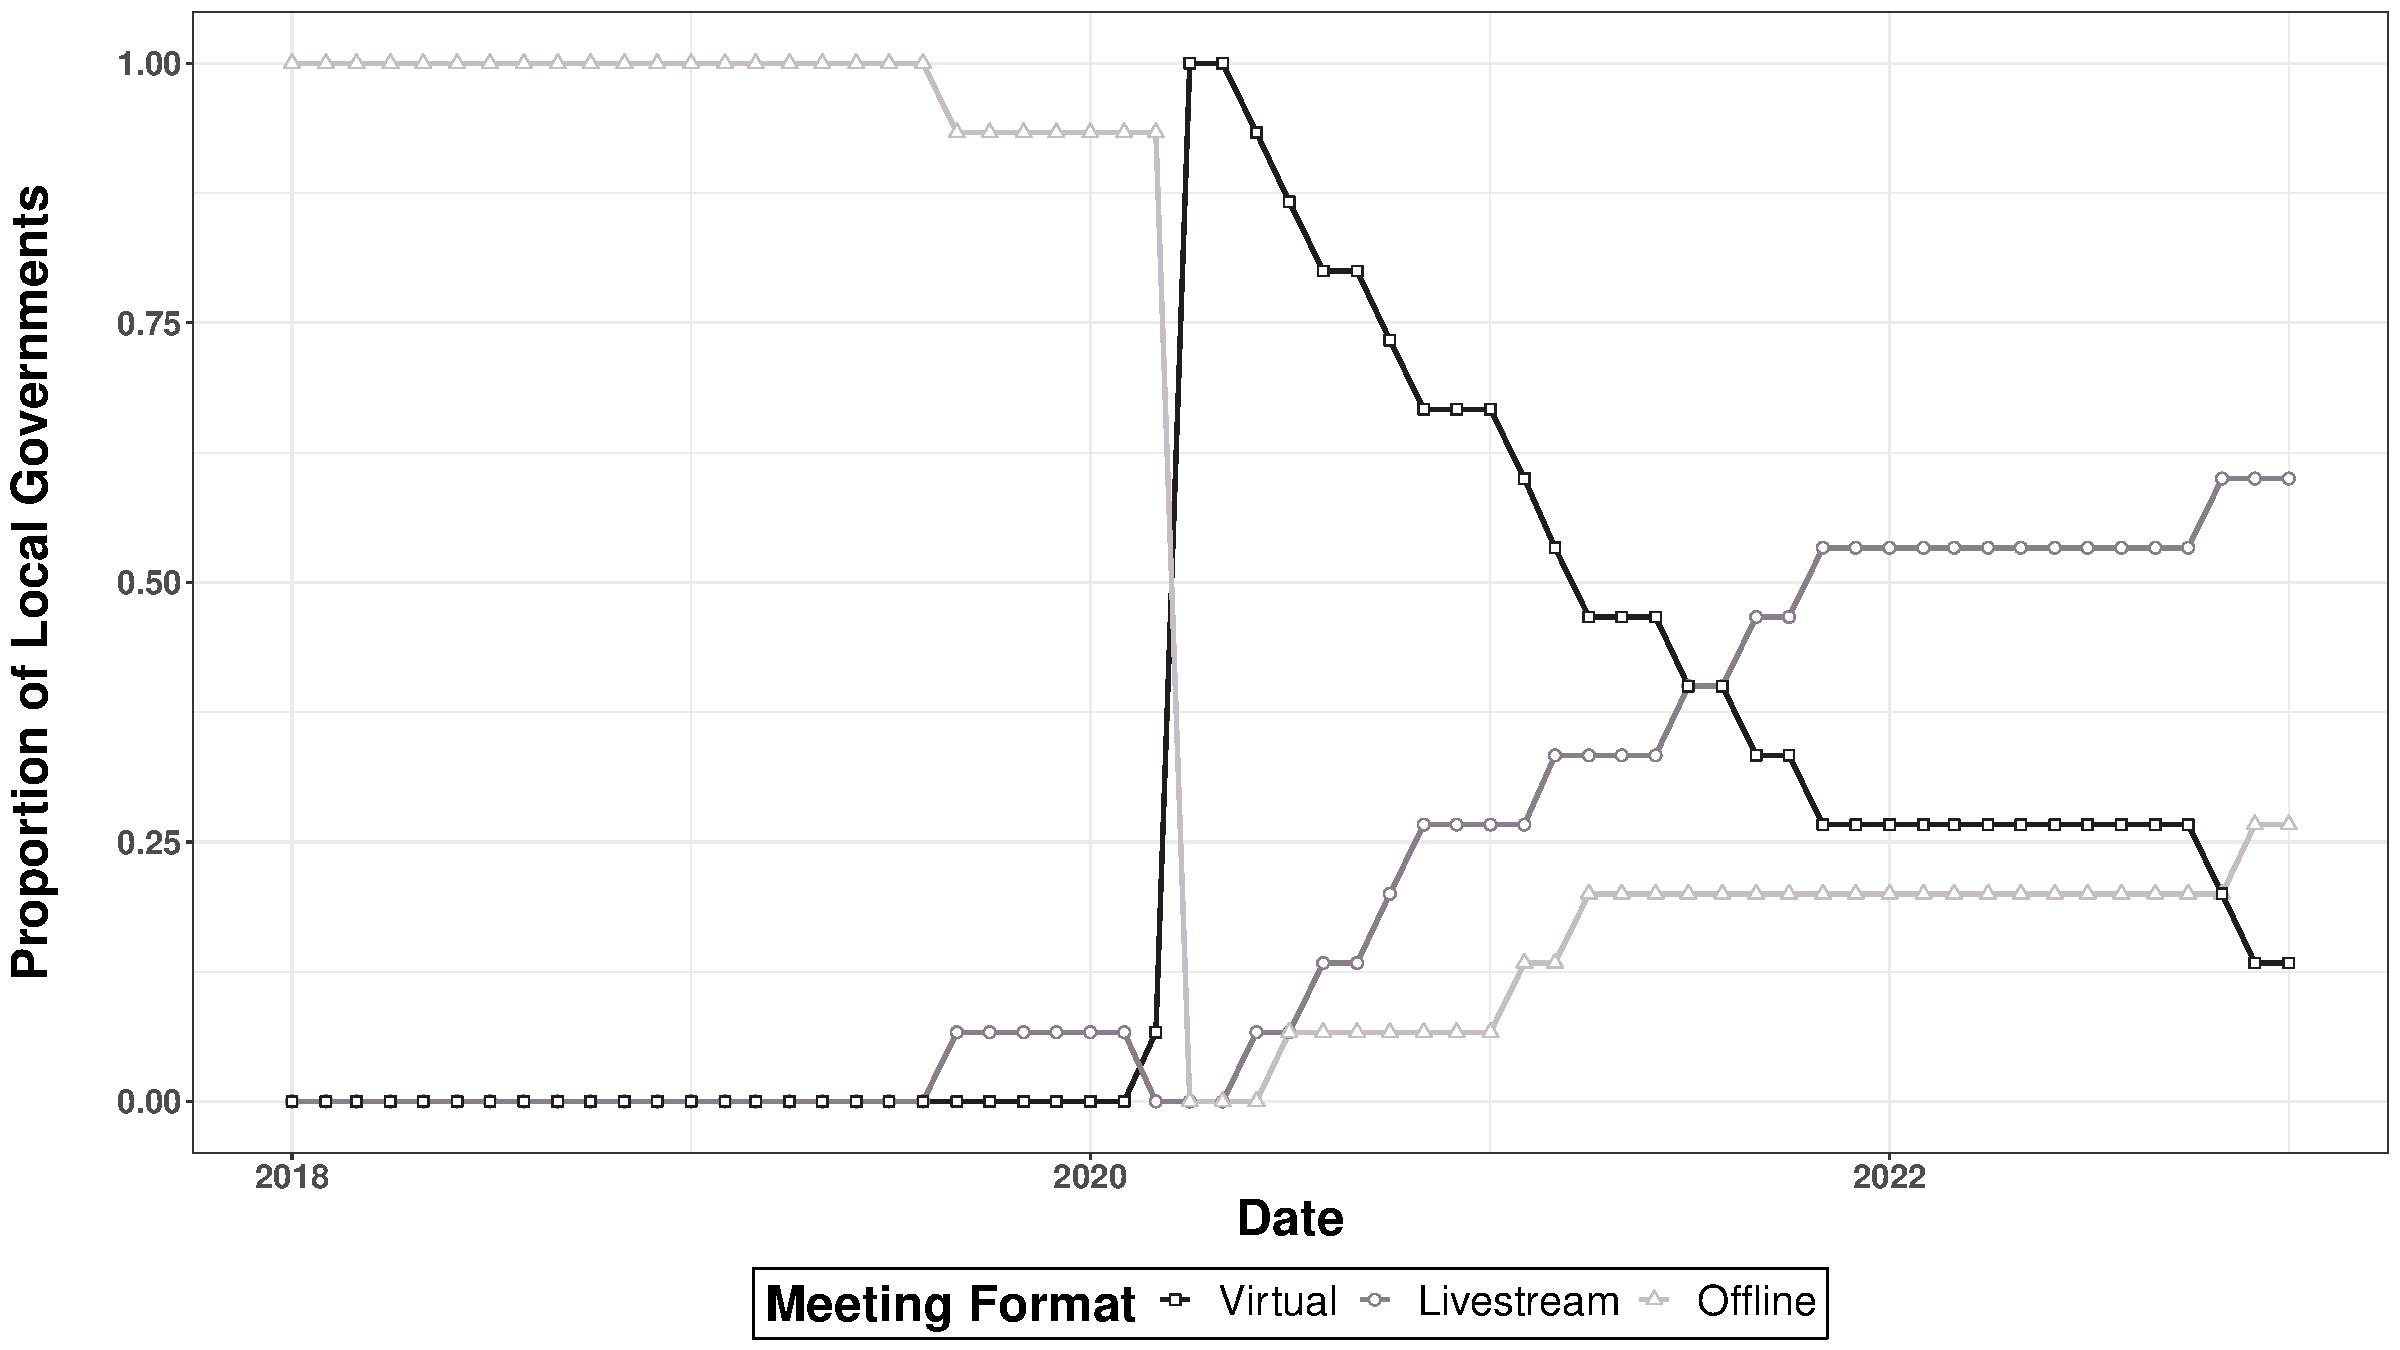
\includegraphics[scale=0.3]{Figures/SchoolAccess.pdf}
    \caption[Access to School Board Meetings From 2018-2022]{\footnotesize{}}
    \label{}
\end{figure}

\begin{figure}[H]
  \centering
   \text{Access to County Council Meetings From 2018-2022}\par\medskip
  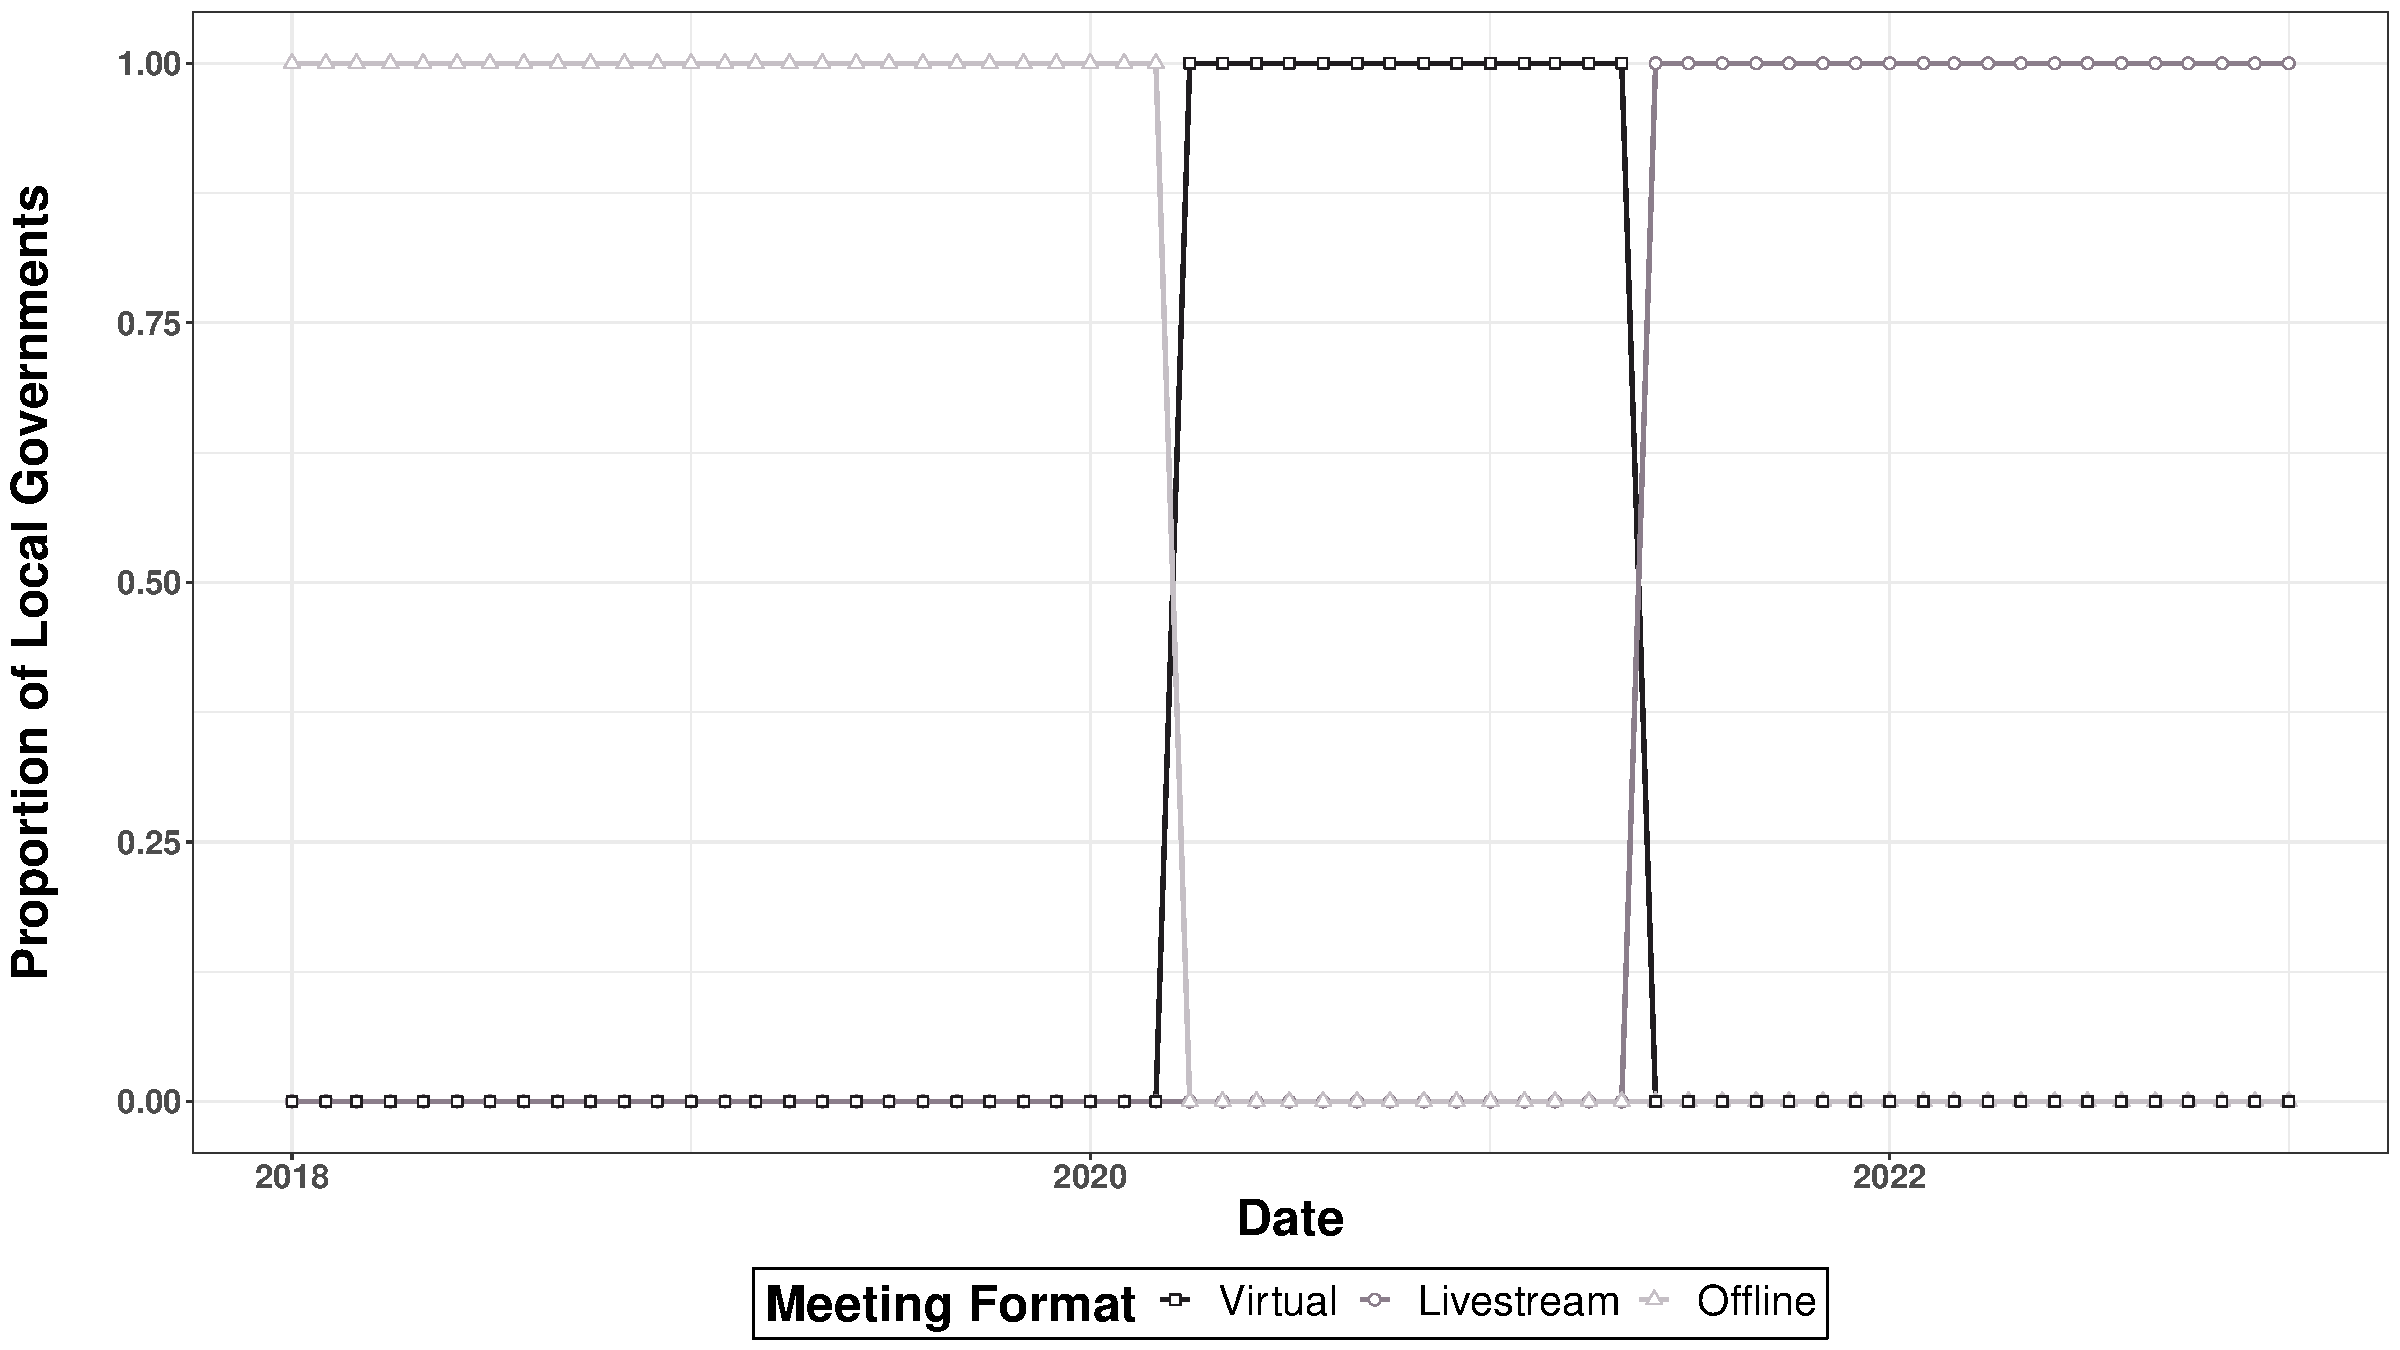
\includegraphics[scale=0.3]{Figures/CountyAccess.pdf}
  \caption[Access to County Council Meetings From 2018-2022]{\footnotesize{}}
  \label{}
\end{figure}




    \section{Full Tables For Figures:}
    \subsection{Figure 2 Regression Tables:}
    \begin{table}[H] \centering 
      \caption{Full Regression Results for Figure 2: Virtual} 
      \label{} 
      \scalebox{0.75}{\begin{tabular}{@{\extracolsep{5pt}}lcccc} 
    \\[-1.8ex]\hline \\[-1.8ex] 
    \\[-1.8ex] & \multicolumn{4}{c}{\textbf{Number of Commenters}} \\ 
     & \textbf{Pooled} & \textbf{County} & \textbf{School District} & \textbf{City} \\ 
    \hline \\[-1.8ex] 
     Virtual & 0.368$^{*}$ & $-$0.129 & 0.330 & 0.306 \\ 
      & (0.176) & (0.363) & (0.255) & (0.260) \\ 
      Constant & $-$0.968$^{*}$ & 3.707$^{*}$ & $-$1.904$^{*}$ & $-$0.019 \\ 
      & (0.415) & (0.240) & (0.673) & (0.449) \\ 
      \hline \\[-1.8ex] 
     Year FE &  & \ding{51}&  &  \\ 
    Month FE & \ding{51}&  & \ding{51}& \ding{51}\\ 
    Goverment FE & \ding{51}&  & \ding{51}& \ding{51}\\ 
    Num. Gov & 38 & 1 & 22 & 15 \\ 
    N & 1800 & 52 & 780 & 968 \\ 
    AIC & 5421.063 & 550.832 & 2614.811 & 2236.291 \\ 
    \hline \\[-1.8ex] 
    \multicolumn{5}{l}{$^{*}$p$<$0.05} \\ 
    \end{tabular} }
    \end{table} 

    \begin{table}[H] \centering 
      \caption{Full Regression Results for Figure 2: Livestreamed} 
      \label{} 
      \scalebox{0.75}{\begin{tabular}{@{\extracolsep{5pt}}lcccc} 
    \\[-1.8ex]\hline \\[-1.8ex] 
    \\[-1.8ex] & \multicolumn{4}{c}{\textbf{Number of Commenters}} \\ 
     & \textbf{Pooled} & \textbf{County} & \textbf{School District} & \textbf{City} \\ 
    \hline \\[-1.8ex] 
     Livestreamed & $-$0.137 & 1.139$^{*}$ & $-$0.363 & 0.261 \\ 
      & (0.178) & (0.528) & (0.256) & (0.290) \\ 
      Constant & $-$0.998$^{*}$ & 3.707$^{*}$ & $-$1.882$^{*}$ & $-$0.017 \\ 
      & (0.419) & (0.261) & (0.674) & (0.449) \\ \\
    \hline \\[-1.8ex] 
     Year FE &  & \ding{51}&  &  \\ 
    Month FE & \ding{51}&  & \ding{51}& \ding{51}\\ 
    Goverment FE & \ding{51}&  & \ding{51}& \ding{51}\\ 
    Num. Gov & 38 & 1 & 22 & 15 \\ 
    N & 1800 & 52 & 780 & 968 \\ 
    AIC & 5434.779 & 564.507 & 2614.505 & 2236.835 \\ 
    \hline \\[-1.8ex] 
    \multicolumn{5}{l}{$^{*}$p$<$0.05} \\ 
    \end{tabular} }
    \end{table} 

    \begin{table}[H] \centering 
      \caption{Full Regression Results for Figure 2: Online} 
      \label{} 
      \scalebox{0.75}{\begin{tabular}{@{\extracolsep{5pt}}lcccc} 
    \\[-1.8ex]\hline \\[-1.8ex] 
    \\[-1.8ex] & \multicolumn{4}{c}{\textbf{Number of Commenters}} \\ 
     & \textbf{Pooled} & \textbf{County} & \textbf{School District} & \textbf{City} \\ 
    \hline \\[-1.8ex] 
     Online & 0.246 & 2.483$^{*}$ & $-$0.050 & 0.293 \\ 
      & (0.181) & (0.566) & (0.346) & (0.203) \\ 
      Constant & $-$1.048$^{*}$ & 3.707$^{*}$ & $-$1.941$^{*}$ & $-$0.004 \\ 
      & (0.419) & (0.247) & (0.675) & (0.449) \\ \\
    \hline \\[-1.8ex] 
     Year FE &  & \ding{51}&  &  \\ 
    Month FE & \ding{51}&  & \ding{51}& \ding{51}\\ 
    Goverment FE & \ding{51}&  & \ding{51}& \ding{51}\\ 
    Num. Gov & 38 & 1 & 22 & 15 \\ 
    N & 1800 & 52 & 780 & 968 \\ 
    AIC & 5433.647 & 557.457 & 2616.083 & 2235.560 \\ 
    \hline \\[-1.8ex] 
    \multicolumn{5}{l}{$^{*}$p$<$0.05} \\ 
    \end{tabular} }
    \end{table} 



    \subsection{Figure 3 Regression Tables}
    \begin{table}[H]
      \centering
      \caption{Full Regession Results of Switching Away from Virtual Meetings}
      \scalebox{0.75}{\begin{tabular}{lccc}
        \hline\\[-1.8ex]
        \textbf{Group} & \textbf{Estimate} & \textbf{Std. Error} & \textbf{[95\% Pointwise Conf. Band]} \\
      \hline\\[-1.8ex]
      2 & -6.0815 & 1.8841 & [-9.7743, -2.3886]* \\
      3 & 4.4265 & 7.9697 & [-11.1939, 20.0469] \\
      4 & -8.5765 & 2.5928 & [-13.6583, -3.4946]* \\
      6 & -29.9583 & 3.5539 & [-36.9239, -22.9927]* \\
      7 & 1.4810 & 5.0879 & [-8.4911, 11.4530] \\
      10 & -2.0547 & 1.6289 & [-5.2472, 1.1378] \\
      11 & 1.4188 & 2.4016 & [-3.2883, 6.1259] \\
      13 & -0.7655 & 1.3506 & [-3.4126, 1.8816] \\
      15 & -0.4200 & 1.4075 & [-3.1786, 2.3386] \\
      17 & 4.6250 & 2.8540 & [-0.9688, 10.2188] \\
      19 & -11.5000 & 0.7413 & [-12.9529, -10.0471]* \\
      \hline 
      \hline
      \end{tabular}}
      \end{table}

      \begin{table}[H]
        \centering
        \caption{Full Regession Results of Switching Away from Online Meetings}
        \scalebox{0.75}{\begin{tabular}{lccc}
          \hline\\[-1.8ex]
          \textbf{Group} & \textbf{Estimate} & \textbf{Std. Error} & \textbf{[95\% Pointwise Conf. Band]} \\
        \hline\\[-1.8ex]
        3 & 1.2063 & 4.3231 & [-7.2669, 9.6794] \\
        10 & -2.6389 & 1.8715 & [-6.3070, 1.0292] \\
        13 & -2.5486 & 2.1956 & [-6.8519, 1.7547] \\
        \hline 
        \hline
        \end{tabular}}
        \end{table}
      


    \subsection{Figure 4 Regression Tables}
    \begin{table}[H]
      \centering
      \caption{Full Regession Results of Switching Away from Virtual Meetings}
      \scalebox{0.75}{\begin{tabular}{lccc}
        \hline\\[-1.8ex]
        \textbf{Group} & \textbf{Estimate} & \textbf{Std. Error} & \textbf{[95\% Pointwise Conf. Band]} \\
      \hline\\[-1.8ex]
      2 & -0.4765 & 0.9735 & [-2.4581, 1.5051] \\
      6 & 1.1591 & 0.2685 & [0.6124, 1.7057]* \\
      12 & 1.1461 & 0.3533 & [0.4270, 1.8652]* \\
      13 & -0.1097 & 0.4969 & [-1.1213, 0.9018] \\
      14 & -0.7552 & 0.7571 & [-2.2964, 0.7859] \\
      15 & 1.0909 & 1.4397 & [-1.8398, 4.0216] \\
      \hline 
      \hline
      \end{tabular}}
      \end{table}

    \begin{table}[H]
        \centering
        \caption{Full Regession Results of Switching Away from Online Meetings}
        \scalebox{0.75}{\begin{tabular}{lccc}
          \hline\\[-1.8ex]
          \textbf{Group} & \textbf{Estimate} & \textbf{Std. Error} & \textbf{[95\% Pointwise Conf. Band]} \\
        \hline\\[-1.8ex]
        2 & -0.4508 & 1.0045 & [-2.4292, 1.5276] \\
        6 & 1.2019 & 0.2565 & [0.6967, 1.7071]* \\
        12 & 1.2030 & 0.3007 & [0.6107, 1.7953]* \\
        13 & -0.2583 & 0.3845 & [-1.0156, 0.4990] \\
        15 & 0.7000 & 1.1169 & [-1.4998, 2.8998] \\
        \hline 
        \hline
        \end{tabular}}
        \end{table}

    \section{Supplementary Analyses:}
    \subsection{Simultaneous Comparisons of Commenters to Voters}
    \begin{table}[H] \centering 
      \caption{Pooled Commenters Compared to Voters} 
      \label{} 
    \scalebox{0.75}{\begin{tabular}{@{\extracolsep{5pt}}lcccc} 
    \\[-1.8ex]\hline 
    \hline \\[-1.8ex] 
     & \multicolumn{4}{c}{\textit{Dependent variable:}} \\ 
    \cline{2-5} 
    \\[-1.8ex] 
     & Pooled & County & City & School \\ 
    \\[-1.8ex] & (1) & (2) & (3) & (4)\\ 
    \hline \\[-1.8ex] 
     White & 0.177$^{*}$ & 0.154 & 0.259$^{*}$ & 0.106 \\ 
      & (0.062) & (0.081) & (0.128) & (0.149) \\ 
      & & & & \\ 
     Black & $-$0.089 & $-$0.028 & $-$0.493 & $-$0.144 \\ 
      & (0.121) & (0.164) & (0.378) & (0.219) \\ 
      & & & & \\ 
     Gender (F) & 0.492$^{*}$ & 0.760$^{*}$ & $-$0.171 & 0.805$^{*}$ \\ 
      & (0.046) & (0.064) & (0.088) & (0.120) \\ 
      & & & & \\ 
     Income (100K+) & 0.247$^{*}$ & 0.305$^{*}$ & 0.029 & 0.443$^{*}$ \\ 
      & (0.047) & (0.062) & (0.094) & (0.117) \\ 
      & & & & \\ 
     Education (HS+) & $-$0.048 & $-$0.068 & 0.157 & $-$0.172 \\ 
      & (0.058) & (0.077) & (0.123) & (0.136) \\ 
      & & & & \\ 
     Homeowner & 0.530$^{*}$ & 0.500$^{*}$ & 0.682$^{*}$ & 0.636$^{*}$ \\ 
      & (0.068) & (0.091) & (0.142) & (0.149) \\ 
      & & & & \\ 
     National Voter & 0.785$^{*}$ & 0.837$^{*}$ & 0.825$^{*}$ & 0.622$^{*}$ \\ 
      & (0.078) & (0.100) & (0.174) & (0.193) \\ 
      & & & & \\ 
     Local Voter & 1.104$^{*}$ & 0.860$^{*}$ & 1.403$^{*}$ & 1.439$^{*}$ \\ 
      & (0.048) & (0.062) & (0.104) & (0.123) \\ 
      & & & & \\ 
     Constant & $-$7.778$^{*}$ & $-$8.083$^{*}$ & $-$8.639$^{*}$ & $-$9.214$^{*}$ \\ 
      & (0.189) & (0.229) & (0.303) & (0.374) \\ 
      & & & & \\ 
    \hline \\[-1.8ex] 
    Zipcode FE & \ding{51}& \ding{51}& - & - \\ 
    City FE & - & - & \ding{51}& - \\ 
    School FE & - & - & - & \ding{51}\\ 
    Observations & 632,187 & 632,187 & 171,772 & 327,165 \\ 
    Akaike Inf. Crit. & 25,908.220 & 16,388.060 & 6,302.015 & 4,858.056 \\ 
    \hline 
    \hline \\[-1.8ex] 
    \textit{Note:}  & \multicolumn{4}{r}{$^{*}$p$<$0.05} \\ 
    \end{tabular} }
    \end{table} 

    \begin{table}[H] \centering 
      \caption{Online and Offline Commenters Compared to All Voters} 
      \label{} 
    \scalebox{0.75}{\begin{tabular}{@{\extracolsep{5pt}}lcccccccc} 
    \\[-1.8ex]\hline 
    \hline \\[-1.8ex] 
     & \multicolumn{8}{c}{\textit{Dependent variable:}} \\ 
    \cline{2-9} 
    \\[-1.8ex] 
     & \multicolumn{2}{c}{Pooled} & \multicolumn{2}{c}{County} & \multicolumn{2}{c}{City} & \multicolumn{2}{c}{School} \\ 
     
    \\[-1.8ex] & (Online) & (Offline) & (Online) & (Offline) & (Online) & (Offline) & (Online) & (Offline)\\ 
    \hline \\[-1.8ex] 
     White & 0.149 & 0.253$^{*}$ & 0.097 & 0.474$^{*}$ & 0.409 & 0.230 & 0.319 & $-$0.106 \\ 
      & (0.077) & (0.109) & (0.087) & (0.220) & (0.246) & (0.159) & (0.218) & (0.209) \\ 
      & & & & & & & & \\ 
     Black & $-$0.189 & 0.105 & $-$0.128 & 0.333 & $-$0.046 & $-$0.701 & $-$0.218 & 0.018 \\ 
      & (0.159) & (0.193) & (0.201) & (0.315) & (0.558) & (0.527) & (0.305) & (0.339) \\ 
      & & & & & & & & \\ 
     Gender (F) & 0.792$^{*}$ & 0.059 & 0.942$^{*}$ & 0.043 & $-$0.224 & $-$0.076 & 1.073$^{*}$ & 0.557$^{*}$ \\ 
      & (0.061) & (0.075) & (0.074) & (0.137) & (0.159) & (0.111) & (0.174) & (0.175) \\ 
      & & & & & & & & \\ 
     Income (100K+) & 0.325$^{*}$ & 0.130 & 0.383$^{*}$ & $-$0.100 & $-$0.080 & 0.133 & 0.351$^{*}$ & 0.531$^{*}$ \\ 
      & (0.059) & (0.082) & (0.068) & (0.158) & (0.172) & (0.119) & (0.158) & (0.177) \\ 
      & & & & & & & & \\ 
     Education (HS+) & $-$0.092 & 0.056 & $-$0.110 & 0.137 & 0.208 & 0.146 & $-$0.236 & $-$0.017 \\ 
      & (0.072) & (0.101) & (0.084) & (0.192) & (0.223) & (0.155) & (0.180) & (0.217) \\ 
      & & & & & & & & \\ 
     Homeowner & 0.577$^{*}$ & 0.411$^{*}$ & 0.590$^{*}$ & 0.181 & 0.630$^{*}$ & 0.658$^{*}$ & 0.624$^{*}$ & 0.667$^{*}$ \\ 
      & (0.087) & (0.109) & (0.105) & (0.181) & (0.242) & (0.180) & (0.200) & (0.233) \\ 
      & & & & & & & & \\ 
     National Voter & 0.755$^{*}$ & 0.849$^{*}$ & 0.778$^{*}$ & 1.145$^{*}$ & 0.778$^{*}$ & 0.907$^{*}$ & 0.650$^{*}$ & 0.538 \\ 
      & (0.094) & (0.144) & (0.108) & (0.259) & (0.296) & (0.228) & (0.246) & (0.324) \\ 
      & & & & & & & & \\ 
     Local Voter & 0.903$^{*}$ & 1.443$^{*}$ & 0.801$^{*}$ & 1.127$^{*}$ & 1.228$^{*}$ & 1.407$^{*}$ & 1.150$^{*}$ & 1.908$^{*}$ \\ 
      & (0.060) & (0.087) & (0.069) & (0.149) & (0.182) & (0.132) & (0.158) & (0.209) \\ 
      & & & & & & & & \\ 
     Constant & $-$8.088$^{*}$ & $-$9.405$^{*}$ & $-$8.183$^{*}$ & $-$24.595 & $-$10.272$^{*}$ & $-$9.290$^{*}$ & $-$9.580$^{*}$ & $-$10.911$^{*}$ \\ 
      & (0.222) & (0.391) & (0.241) & (410.557) & (0.600) & (0.391) & (0.469) & (0.717) \\ 
      & & & & & & & & \\ 
    \hline \\[-1.8ex] 
    Zipcode FE & \ding{51}& \ding{51}& \ding{51}& \ding{51}& - & - & - & - \\ 
    City FE & - & - & - & - & \ding{51}& \ding{51}& - & - \\ 
    School FE & - & - & - & - & - & - & \ding{51}& \ding{51}\\ 
    Observations & 632,187 & 632,187 & 632,187 & 632,187 & 171,772 & 171,772 & 327,165 & 327,165 \\ 
    Akaike Inf. Crit. & 17,646.340 & 10,154.080 & 13,628.920 & 3,802.738 & 2,261.061 & 4,212.815 & 2,921.446 & 2,248.457 \\ 
    \hline 
    \hline \\[-1.8ex] 
    \textit{Note:}  & \multicolumn{8}{r}{$^{*}$p$<$0.05} \\ 
    \end{tabular} }
    \end{table} 


    


    \section{Text-Analysis of Comments}
    \subsection{Examining the Content of Public Meeting Comments}
    In the following section I construct a separate STM model (K=20) for each level government within my sample (Roberts et al. 2019). Each model includes government and month level controls. For the county model, I replace government controls with zipcode controls. \autoref{tab:STMFull} presents the top 5 topics for each level of government.

    \begin{table}[H]
        \centering
        \caption{STM: Comment Topics By Level of Government}
        \label{tab:STMFull}
        \scalebox{.8}{
      \begin{tabular}{lll}
          \\[-1.8ex]\hline 
              \hline \\[-1.8ex] 
          \textbf{County Council}                            & \textbf{Municipal Council}                     & \textbf{School Board}                           \\
          \hline \\
          mask, mandat, counti,        & develop, light,       & comment, school,    \\
          wear, vaccin                 & traffic, concern      & chromebook, instruct \\ \\[-1.8ex]
          \hline\\
          sport, counti,        & spoke, propos,   & earn, virtual,  \\
          youth, page, support  & opposit, favor, rezon   & person, graduat, shorten\\ \\[-1.8ex]
          \hline\\
          school, kid,          & contract, renew,          & propos, oppos,     \\
          play, children, team & trash, waste & rezon, concern, spoke \\ \\[-1.8ex]
          \hline\\
          prosecuti, judge,  & concern, construct, & return, school,    \\
          attorney, file, process &  express, sidewalk & staff, online, learn \\ \\[-1.8ex]
          \hline\\
          project, develop,      & maryland, trail,        & spoke, regard,  \\
          tax, propos, resid &    thank, event & favor, concern, kirkwood\\ \\[-1.8ex]
          \\[-1.8ex]\hline 
              \hline \\[-1.8ex]                                  
          \end{tabular}
      }
    \end{table}

    
    Next I follow the same procedure but subset each level of my sample by whether a meeting was accessibile online or not. I then reconstruct a model for each subset across each level of government. \autoref{tab:county_online_offline}, \autoref{tab:city_online_offline}, and \autoref{tab:school_online_offline} display the top four topics for online and offline comments at the county, city, and school district levels. While the exact topics change between online and offline meetings, most topics appear jurisdictionally relevant to their respective level of government. 
    
    
    
    \begin{table}[H]
        \centering
        \caption{County Topics of Online Versus Offline Comments}
        \label{tab:county_online_offline}
        \scalebox{0.8}{
        \begin{tabular}{l|l}
        \hline\\
        \textbf{Online} & \textbf{Offline} \\ \\[-1.8ex]
        \hline\\
        mask, mandat, vaccin, counti, pleas & employe, counti, year, work, servic \\
        & \\ \\[-1.8ex]
                  \hline\\
        sport, play, counti, loui, school & anim, volunt, dog, shelter, counti \\
        & \\\\[-1.8ex]
                  \hline\\
        counti, bill, council, page, power & counti, loui, council, execut, meet \\
        & \\\\[-1.8ex]
                  \hline\\
        counti, loui, tax, propos, properti & tax, million, counti, loui, zoo \\
        & \\\\[-1.8ex]
                  \hline
        \end{tabular}}
        
        \end{table}
        
        \begin{table}[H]
        \centering
        \caption{City Topics of Online Versus Offline Comments}
        \label{tab:city_online_offline}
        \scalebox{0.8}{
        \begin{tabular}{l|l}
        \hline\\
        \textbf{Online} & \textbf{Offline} \\ \\[-1.8ex]
        \hline\\
        council, address, street, highland, terrac & spoke, propos, opposit, comment, concern \\
        & \\ \\[-1.8ex]
                  \hline\\
        state, propos, oppos, develop, favor & develop, concern, oppos, state, traffic \\
        & \\\\[-1.8ex]
                  \hline\\
        van, mark, way, space, rezon & ask, council, citi, servic, note, approach \\
        & \\\\[-1.8ex]
                  \hline\\
        food, unhous, support, mini, pantri & polic, protest, charg, galleria, peac \\
        & \\\\[-1.8ex]
                  \hline
        \end{tabular}}
        
        \end{table}
        
        \begin{table}[H]
        \centering
        \caption{School Board Topics of Online Versus Offline Comments}
        \label{tab:school_online_offline}
        \scalebox{0.8}{
        \begin{tabular}{l|l}
        \hline\\
        \textbf{Online} & \textbf{Offline} \\ \\[-1.8ex]
        \hline\\
        patron, comment, total, various, read & gender, ident, ave, geyer, kepling \\
        & \\ \\[-1.8ex]
                  \hline\\
        graduat, ask, student, parent, ceremoni & comment, polici, kelli, meet, advoc \\
        & \\\\[-1.8ex]
                  \hline\\
        learn, virtual, comment, return, -person & school, spoke, high, pattonvill, student \\
        & \\\\[-1.8ex]
                  \hline\\
        school, year, plan, involv, back--school & board, educ, spoke, member, regard \\
        & \\\\[-1.8ex]
                  \hline\\
        \end{tabular}}
        
        \end{table}

        \subsection{Do Online Meetings Elicit More Negative Comments?}
        Beyond the topics of the comments, I also examine whether online meetings elicit more negative comments. To analyze this, I calculate each comment's average sentence level VADER sentiment scores and scale it between -1 and 1 \citep{Hutto_Gilbert_2014}. Overall, average sentiment for Offline (0.100) and Online (0.099) meetings are both positive, but not statistically different.


\begin{figure}[H]
    \centering
    \caption{Average Comment Sentiment By Meeting Format}
    \label{fig:Sentiment}
    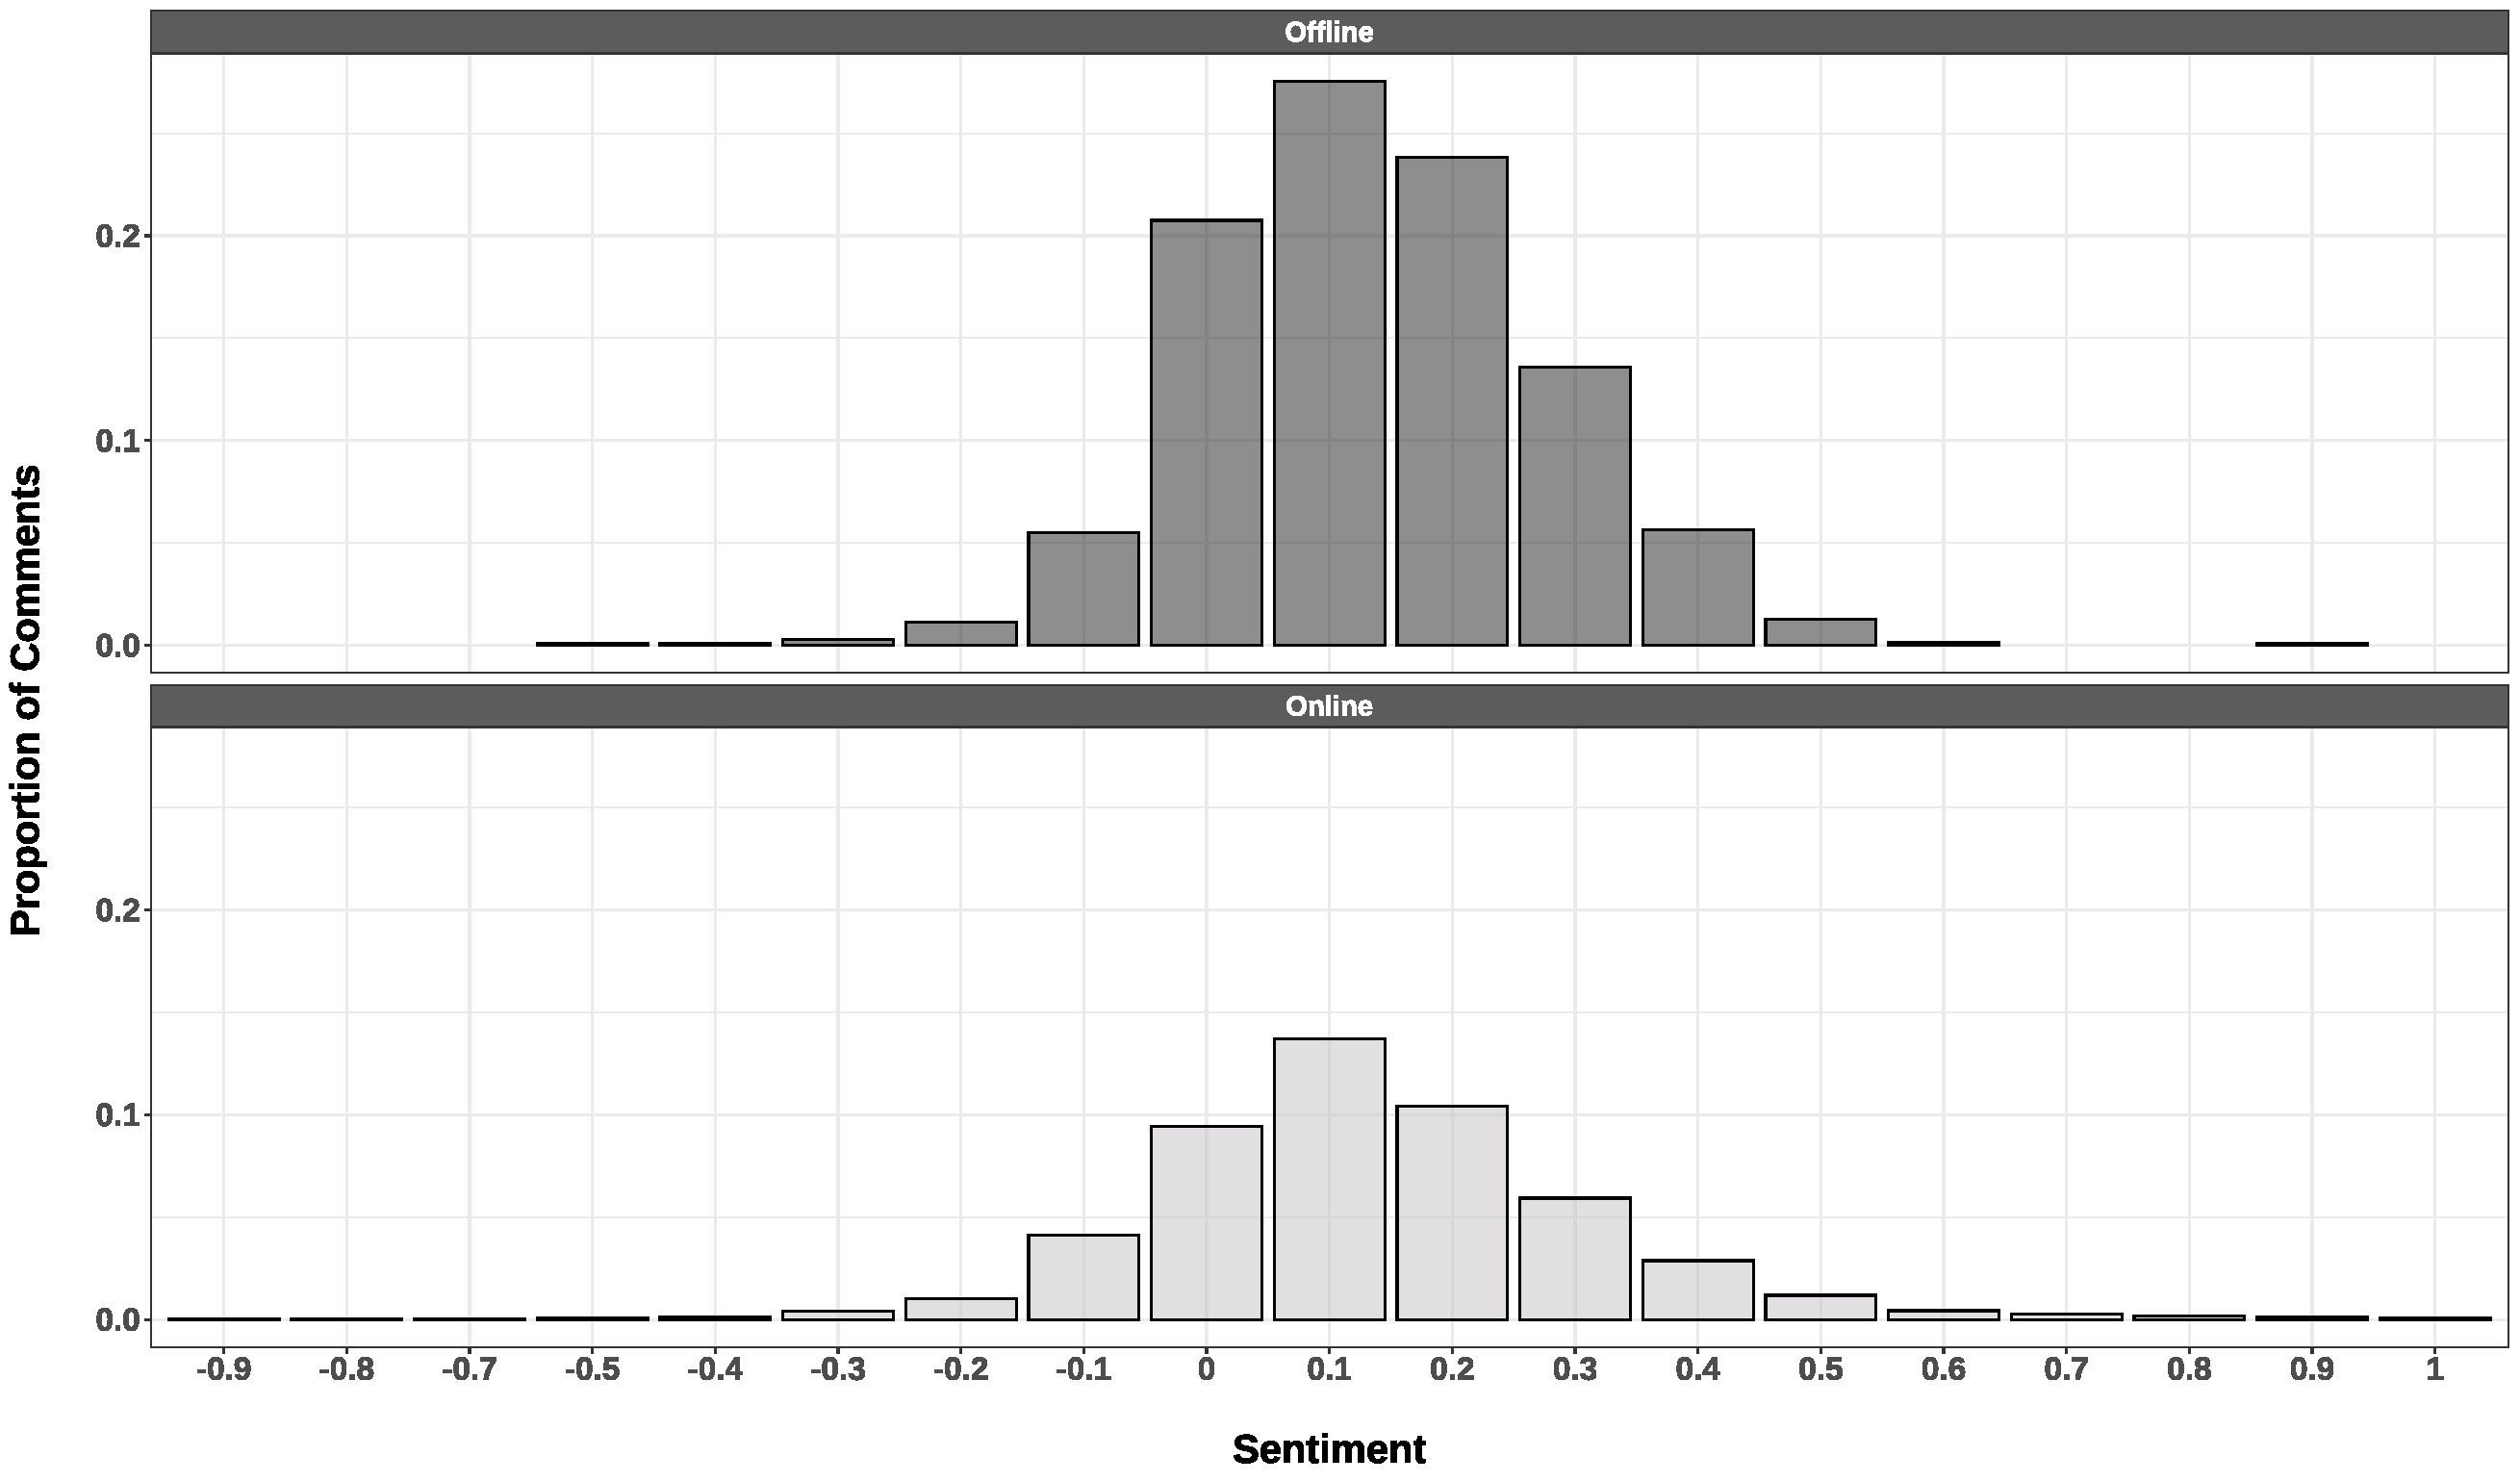
\includegraphics[scale=0.35]{Figures/Sentiment.pdf}
\end{figure}



    
    
    \section{Survey Details:}
    \subsection{Question Wording:}

    \small
      \noindent \textbf{Non-Meeting Attendees:} What best describes why you haven't attended a local political meeting (such as school district or city council) this past year?
      \begin{enumerate}
        \item Inconvenient meeting times
        \item No compelling reason or issue
        \item Unable to join the meeting (either in-person or virtually)
        \item Didn’t know how to attend meetings
        \item Didn’t want to attend meetings alone
        \item Voiced concerns in an alternative way (email, phone call, etc.)
        \item Other (please specify)
      \end{enumerate}


      \noindent \textbf{Meeting Attendees:} What best describes why you attended a local political meeting (such as school district or city council) this past year?
      \begin{enumerate}
        \item Support a specific policy issue.
        \item Oppose a specific policy issue.
        \item Voice an opinion or concern.
        \item Thank a local public official.
        \item Critique a local public official.
        \item Observe the meeting
        \item Other (please specify)
      \end{enumerate}


    \subsection{Survey Responses:}

    \begin{figure}[H]
      \centering
       \text{}\par\medskip
      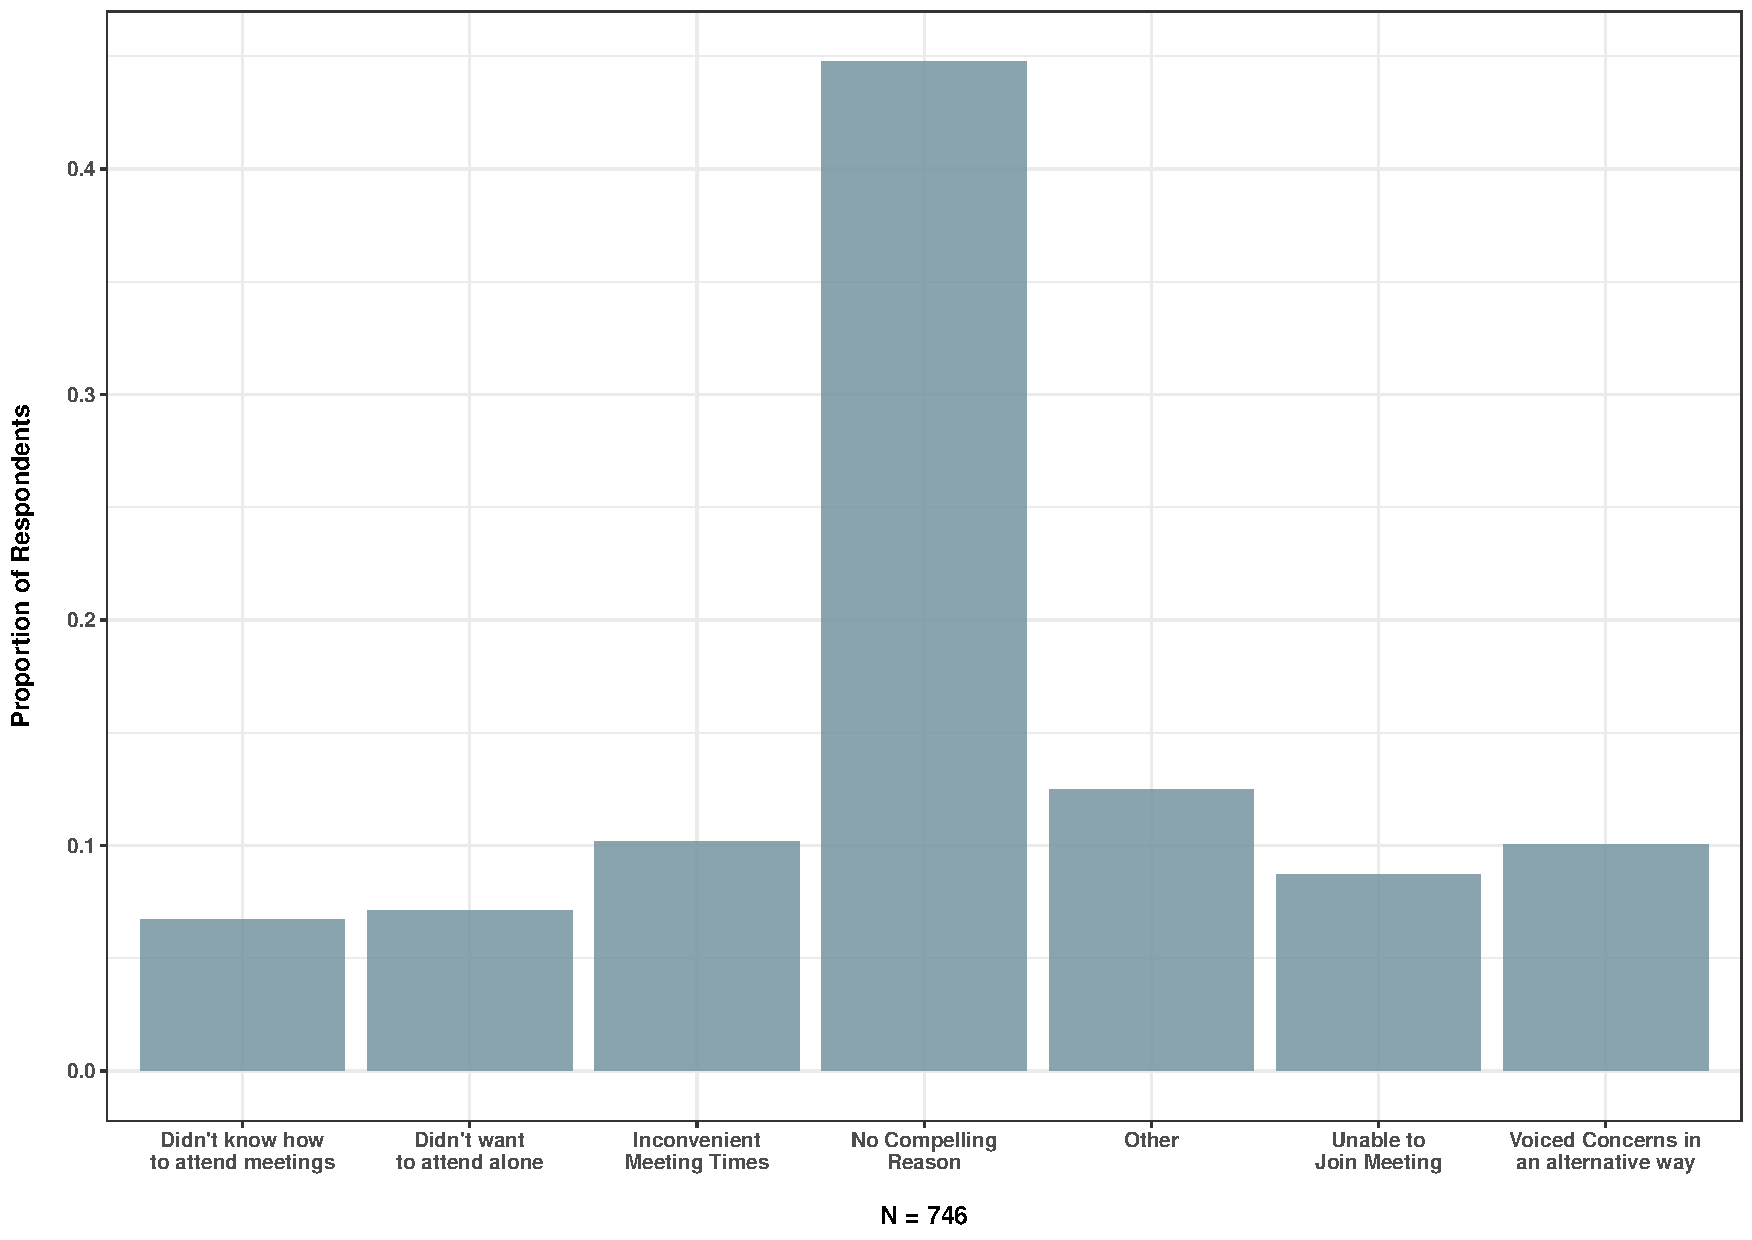
\includegraphics[scale=0.43]{Figures/CCESNoMeeting.pdf}
      \caption[Response to Non-Meeting Attendees Question]{\footnotesize{Response to Non-Meeting Attendees Question}}
      \label{}
    \end{figure}


    \begin{figure}[H]
      \centering
       \text{}\par\medskip
      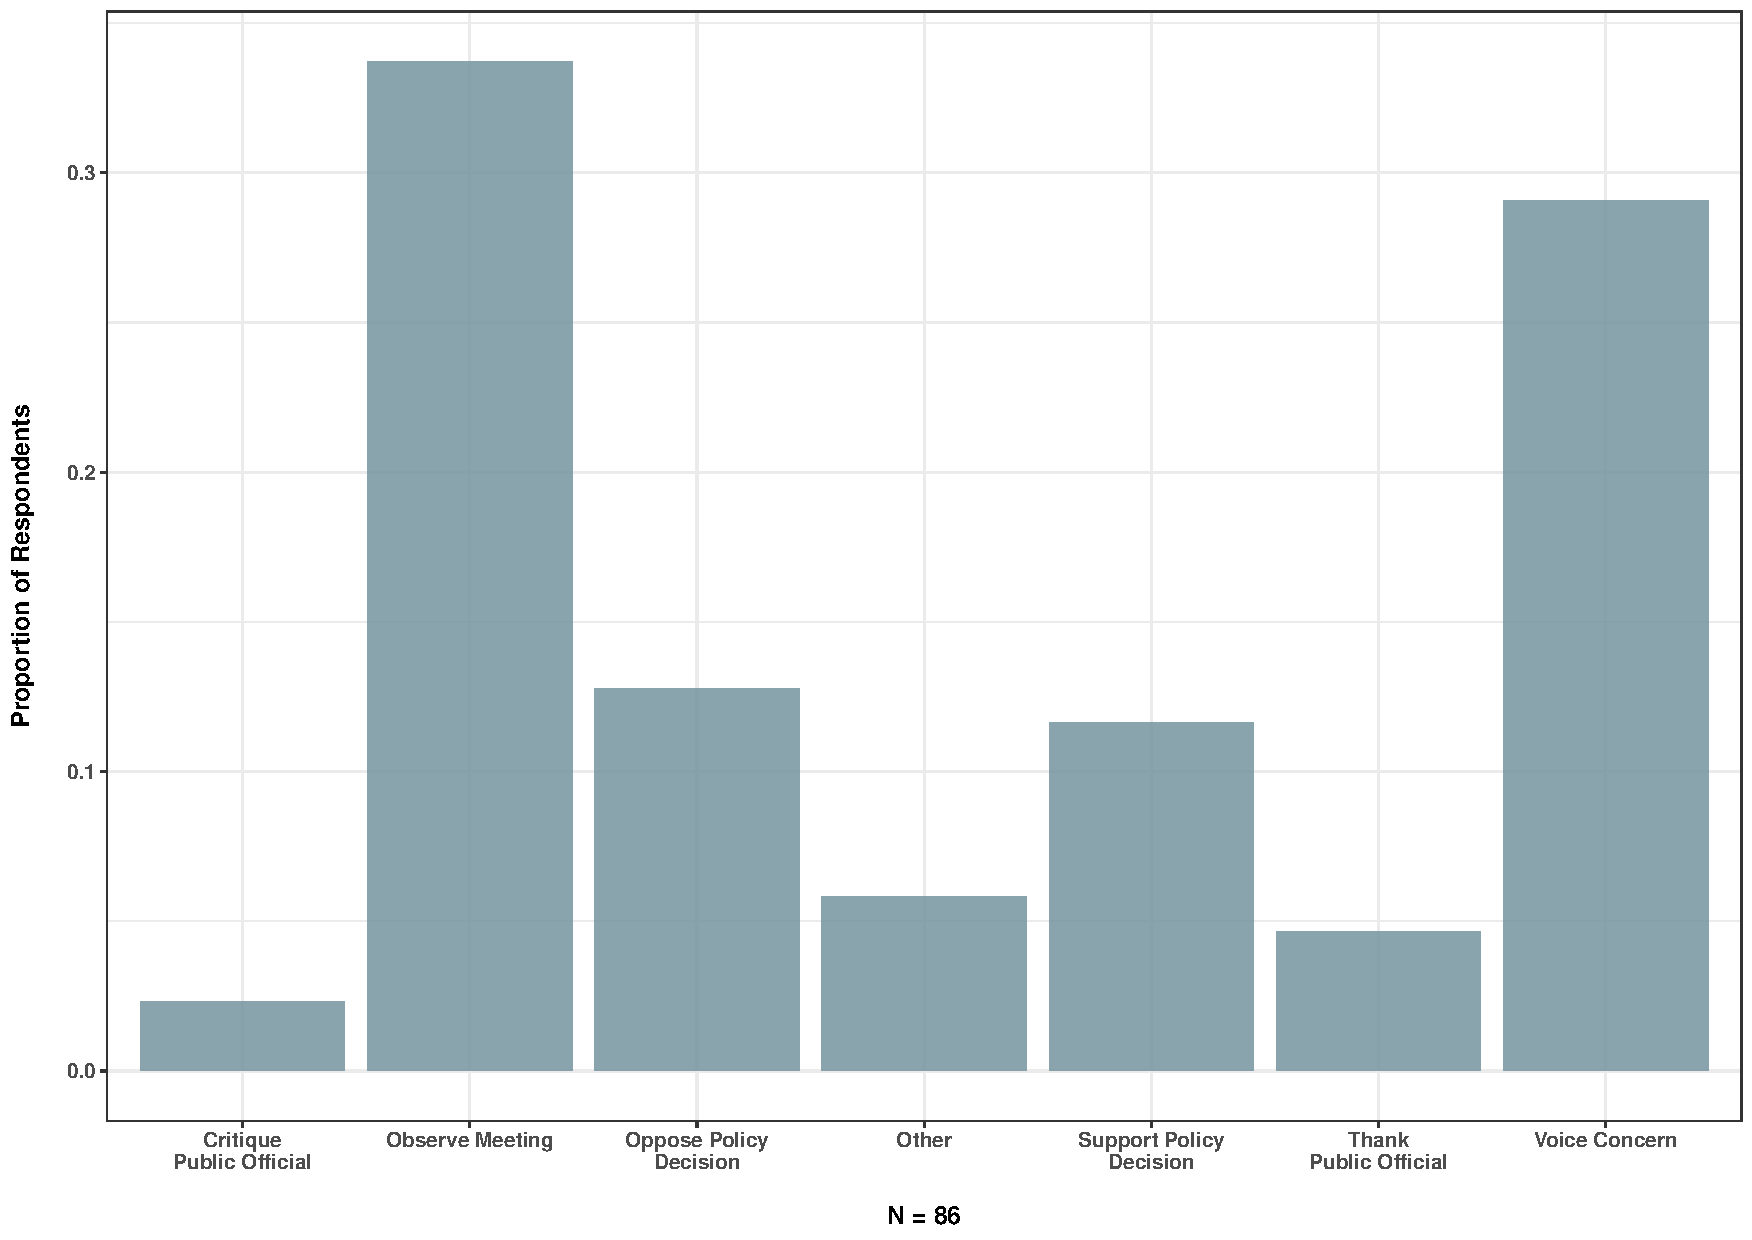
\includegraphics[scale=0.43]{Figures/CCESMeeting.pdf}
      \caption[Response to Meeting Attendees Question]{\footnotesize{Response to Meeting Attendees Question}}
      \label{}
    \end{figure}